\section{Dynamic-MSV-Bench and Methodology}
\label{sec:benchmark}

\begin{figure*}[t]
    \centering
    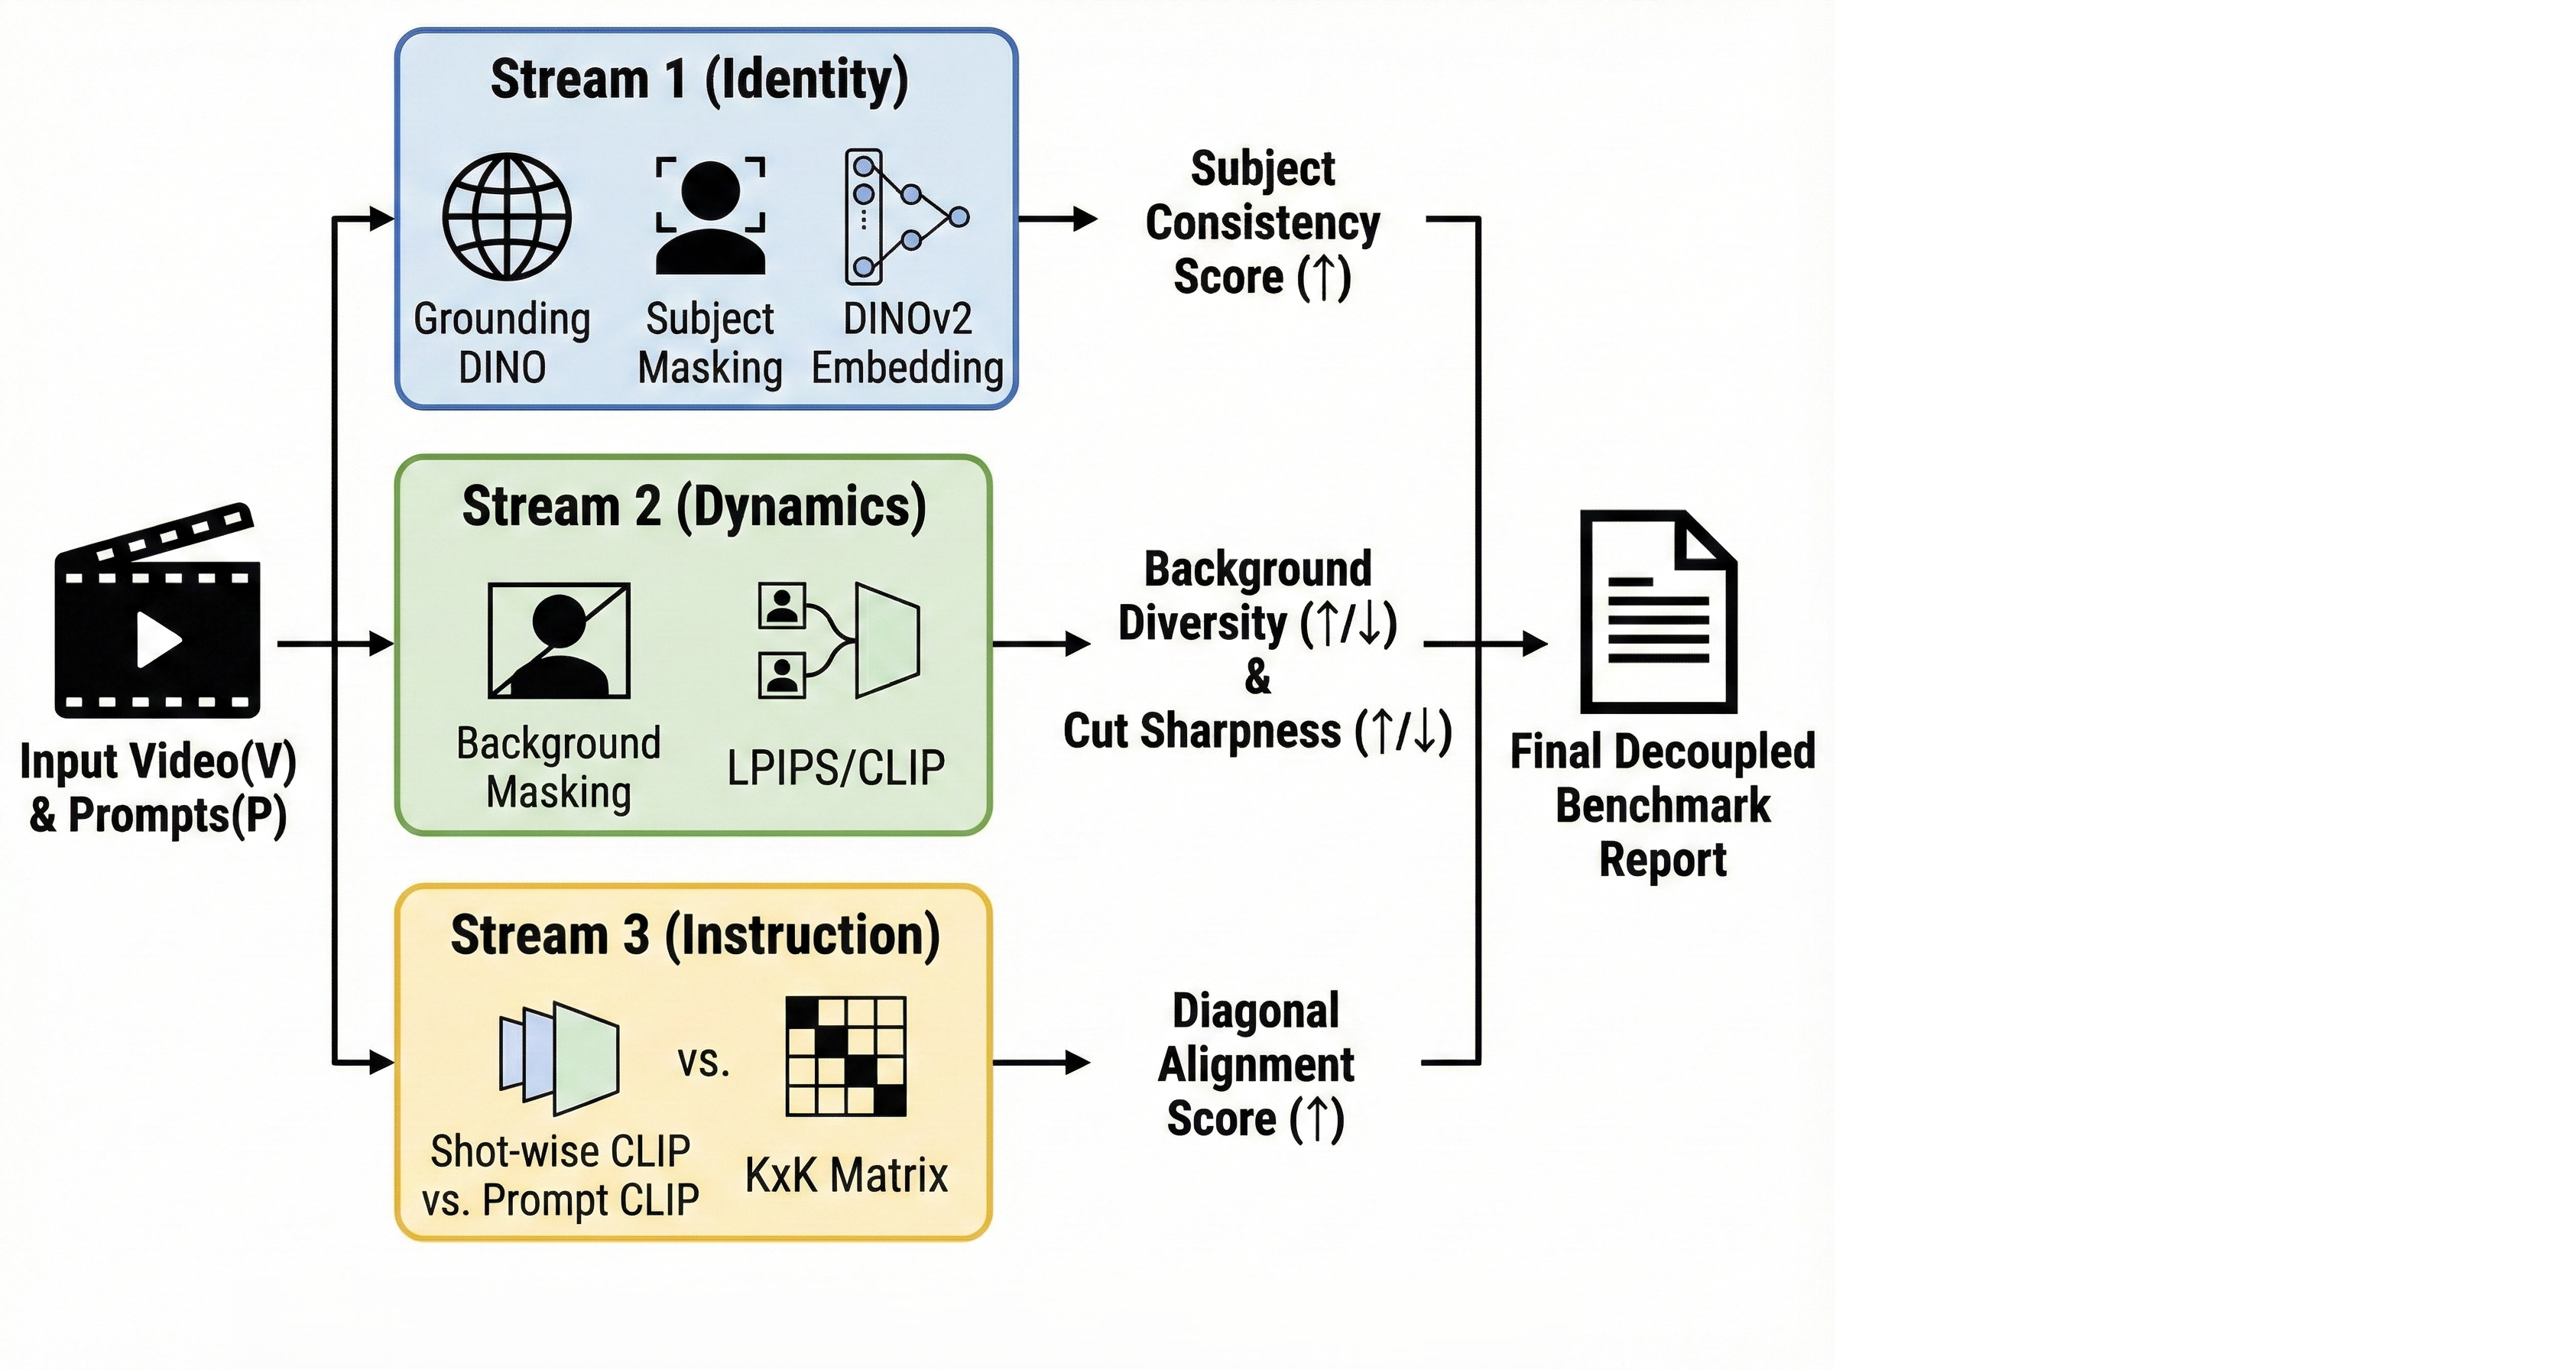
\includegraphics[width=\textwidth]{figures/fig2.png}
    \caption{Overview of our Decoupled 4D Evaluation Framework. Unlike holistic metrics like FVD, we process the input video through three independent streams to measure Subject Identity, Background Dynamics/Continuity, and Instruction Following (Diagonal Alignment) separately. This decoupling allows for scenario-aware evaluation (Set A vs. Set B).}
    \label{fig:framework}
\end{figure*}

\begin{figure*}[t]
    \centering
    \includegraphics[width=\textwidth]{figures/fig_AB.jpg}
    \caption{Conceptual comparison of our two evaluation tracks. (Left) \textbf{Set A: Semantic Shift} requires radical environment changes while preserving the subject, demanding high diversity and sharp cuts. (Right) \textbf{Set B: Motion Control} requires maintaining a consistent background during camera actions (Panning, Zooming, Tracking), demanding low diversity and smooth spatial continuity. Our DSA metric rewards high instruction adherence in both scenarios.}
    \label{fig:sets_comparison}
\end{figure*}

We propose the \textbf{Dynamic-MSV-Bench}, which categorizes multi-shot prompts into two extreme stress-test scenarios to expose the "Double-Kill" dilemma of current models.

\subsection{Track A: Semantic Shift (Narrative Diversity)}
This track evaluates the model's ability to maintain a consistent subject while drastically shifting the semantic environment (e.g., from a dense forest to outer space). 
\textbf{Golden Rule for Track A:} HIGH Subject Consistency, HIGH Background Diversity, HIGH Cut Sharpness, and HIGH Diagonal Alignment. A model that scores low on Diversity here has fallen into the \textbf{Static Trap}.

\subsection{Track B: Motion Control (Spatial Integrity)}
This track tests whether a model can execute continuous physical instructions (e.g., Panning, Zooming) while keeping the background pixel-perfectly stable.
\textbf{Golden Rule for Track B:} HIGH Subject Consistency, LOW Background Diversity, LOW Cut Sharpness, and HIGH Diagonal Alignment. A model that scores high on Diversity here suffers from \textbf{Background Hallucination}.

\subsection{The 4D Decoupled Metrics}
Our framework evaluates videos through three independent streams (Identity, Dynamics, Instruction):
\begin{enumerate}
    \item \textbf{Subject Consistency ($\mathcal{C}_{subj}$):} DINOv2~\cite{oquab2023dinov2} similarity of bounding-box masked subjects across shots.
    \item \textbf{Background Diversity ($\mathcal{D}_{bg}$):} Inverse cosine similarity of the isolated background environment.
    \item \textbf{Cut-Transition Sharpness ($\mathcal{S}_{cut}$):} The peak LPIPS~\cite{zhang2018perceptual} distance at the prompted shot boundaries, penalizing blurry morphing.
    \item \textbf{Diagonal Semantic Alignment (DSA):}
    Our core novelty, DSA, uses a $K \times K$ CLIP~\cite{radford2021learning} similarity matrix $M$ between shots and prompts. To penalize prompt-bleeding and static generation, we apply column-wise softmax with logit scaling $\tau$:
    $$P_{i,j} = \frac{\exp(\tau \cdot M_{i,j})}{\sum_{k=1}^{K} \exp(\tau \cdot M_{k,j})}$$
    $$DSA = \frac{\left( \frac{1}{K} \sum_{i=1}^{K} P_{i,i} \right) - \frac{1}{K}}{1 - \frac{1}{K}}$$
    By subtracting the random baseline expectation ($1/K$), DSA mathematically guarantees a score of $0.0$ for any model stuck in the Static Trap (generating identical shots).
\end{enumerate}
